\problemname{Killing Monsters
}

You are playing your favourite video game Boulder's Gait. Each playthrough of Boulder's Gait happens over several rounds. In each round, you select a single monster to battle. Each monster has a particular payout associated with it. The monsters you choose from and their corresponding payouts are the same in every round. You may battle the same monster multiple times in different rounds, and you will receive the same payout each time you battle them.

Your squad is very picky and only wants to do playthroughs where the total payout across all battles can be evenly divided amongst the members of the squad (call those playthroughs \textit{fair}). For example, consider the following monsters and their payouts. Each of the playthroughs listed are fair if your squad has three members because the total payout can be evenly divided amongst the three members of the squad.

\begin{center}
 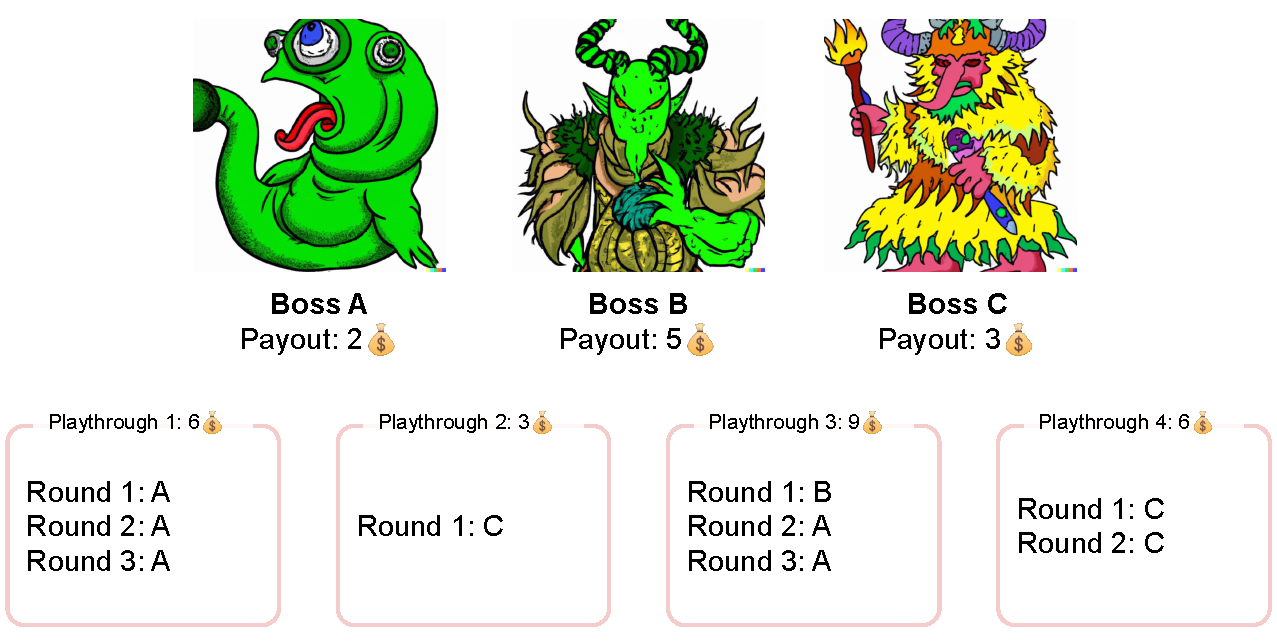
\includegraphics[width=0.8\textwidth]{LootingLuxury}
\end{center}

Two playthroughs are considered the same if they have the exact same number of rounds and the order in which you battle the monsters is identical.

In order for your playthrough to be eligible for the leaderboard, your playthrough must have at least $L$ rounds and at most $U$ rounds.

How many different fair playthroughs are there that are eligible for the leaderboard?


\section*{Input}

The first line of input contains four integers $N$~($1 \leq N \leq 200\,000$), which is the number of monsters to choose from, $K$~($1 \leq K \leq 750$), which is the number of members in your squad, $L$~($1 \leq L \leq 10^9$), which is the minimum number of rounds for your playthrough to be eligible for the leaderboard, and $U$~($L \leq U \leq 10^9$), which is the maximum number of rounds for your playthrough to be eligible for the leaderboard.

The next line contains $N$ integers $b_1, b_2, \dots, b_N$~($1 \leq b_i \leq 10^9$), which are the payouts of the $N$ monsters.


\section*{Output}

Display the number of different fair playthroughs that are eligible for the leaderboard. Display this number modulo $1\,000\,000\,007$.
